\chapter{Strategie 2 (STQA)}

\section{Durchführung (ZB)}

Eine bekannte Wärmebehandlung von $\alpha$+$\beta$-Titanlegierungen ist die  \textit{Solution treatment and quenching + Aging}(Abbildung \ref{fig:SQ}). Im Gegensatz zu  Strategie 1 wird hier ein Duplex-Glühen zum Einstellen eines bi-modalen Gefüges nicht gebraucht. Werkstücke werden im ersten Schritt bei einer Temperatur unterhalb $T_{\beta}$ für 1--2 h geglüht und danach wassergekühlt. Es wurde auch bei dieser Strategie die aus der $\alpha_p$-Studie ermittelte Temperatur von 983$^\circ$C für 60 min gewählt, damit sich vergleichbare $\alpha_p$-Volumenanteile einstellen. Durch das Abschrecken wandelt sich die $\beta$-Phase martensitisch um.

Um das Gefüge noch weiter zu verfeinern, wird der zweite Wärmebehandlungsschritt, das Anlassen, durchgeführt. Hier sollen die Proben nochmal erwärmt und dann luftgekühlt werden. Bei der erhöhten Temperatur soll sich der Martensit in $\beta$- und $\alpha$-Körner umwandeln.
Um beide Strategien noch besser vergleichen zu können werden in diesem Schritt die Proben bei  610$^\circ$C für 16 und 30 min angelassen und anschließend luftgekühlt.

\begin{figure}[h]
	\centering
	{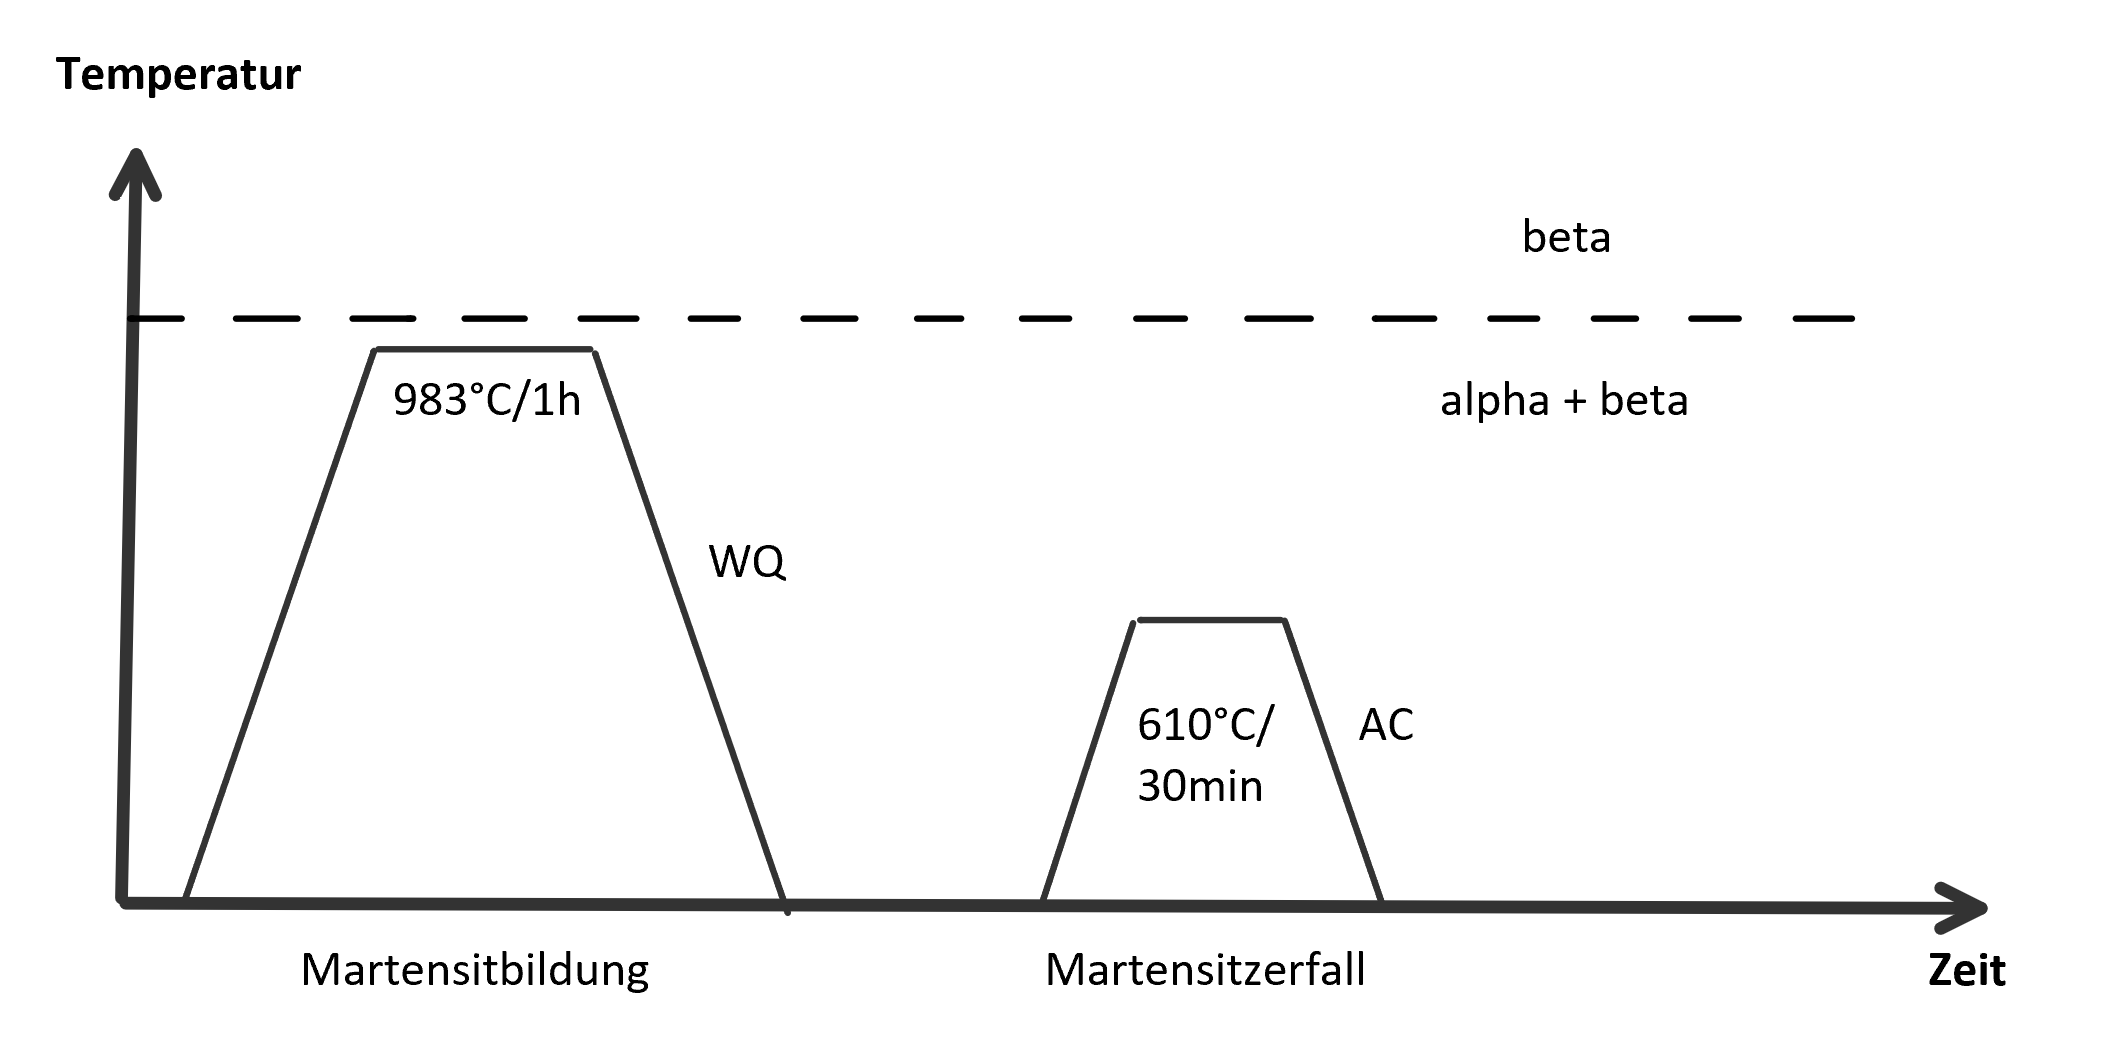
\includegraphics[width=0.9\textwidth]{./Bilder/SQ.png}}
	\caption{Wärmebehandlungsdiagramm von dem Solution Treatment and Quenching + aging}
	\label{fig:SQ}
\end{figure}

\section{Ergebnisse (PH)}

Die durch den ersten Behandlungsschritt entstandene Mikrostruktur wurde unter dem Lichtmikroskop ausgewertet und ist in Abbildung \ref{fig:abbildung-19} aufgeführt.

\begin{figure}[h]
	\centering
	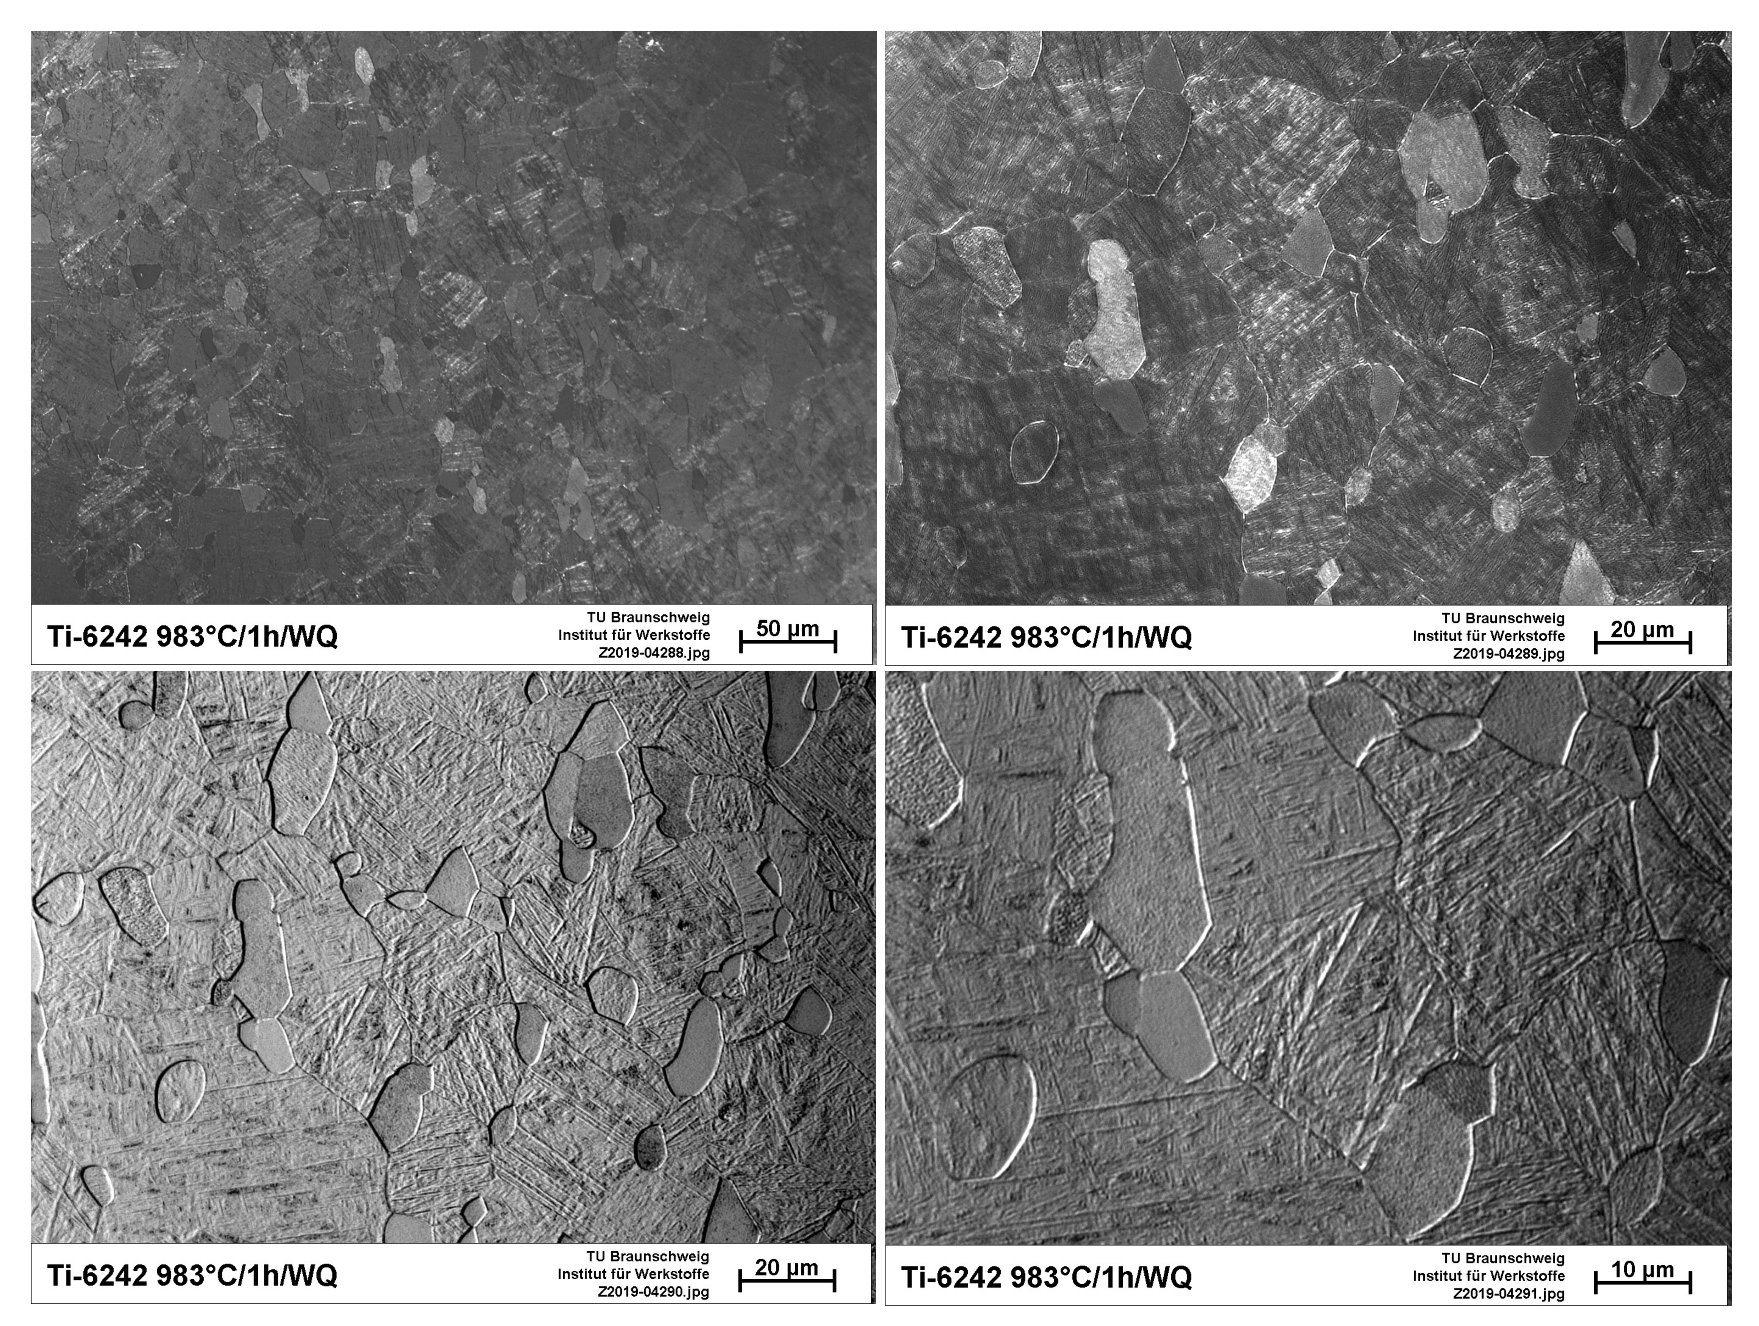
\includegraphics[width=0.9\linewidth]{./Bilder/Abbildung 19.png}
	\caption[Abbildung 19]{$\alpha_p$-$\alpha'$-Gefüge unter dem Lichtmikroskop bei verschiedenen Vergrößerungen (C-DIC)}
	\label{fig:abbildung-19}
\end{figure}

Die anschließende Härteprüfung ergab eine mittlere Vickershärte von 405 HV.

Die Auswertung des zweiten Wärmebehandlungsschritts unter dem REM ist in den Abbildungen \ref{fig:abbildung-26} und \ref{fig:abbildung-27} zusammengefasst.

\begin{figure}[h]
	\centering
	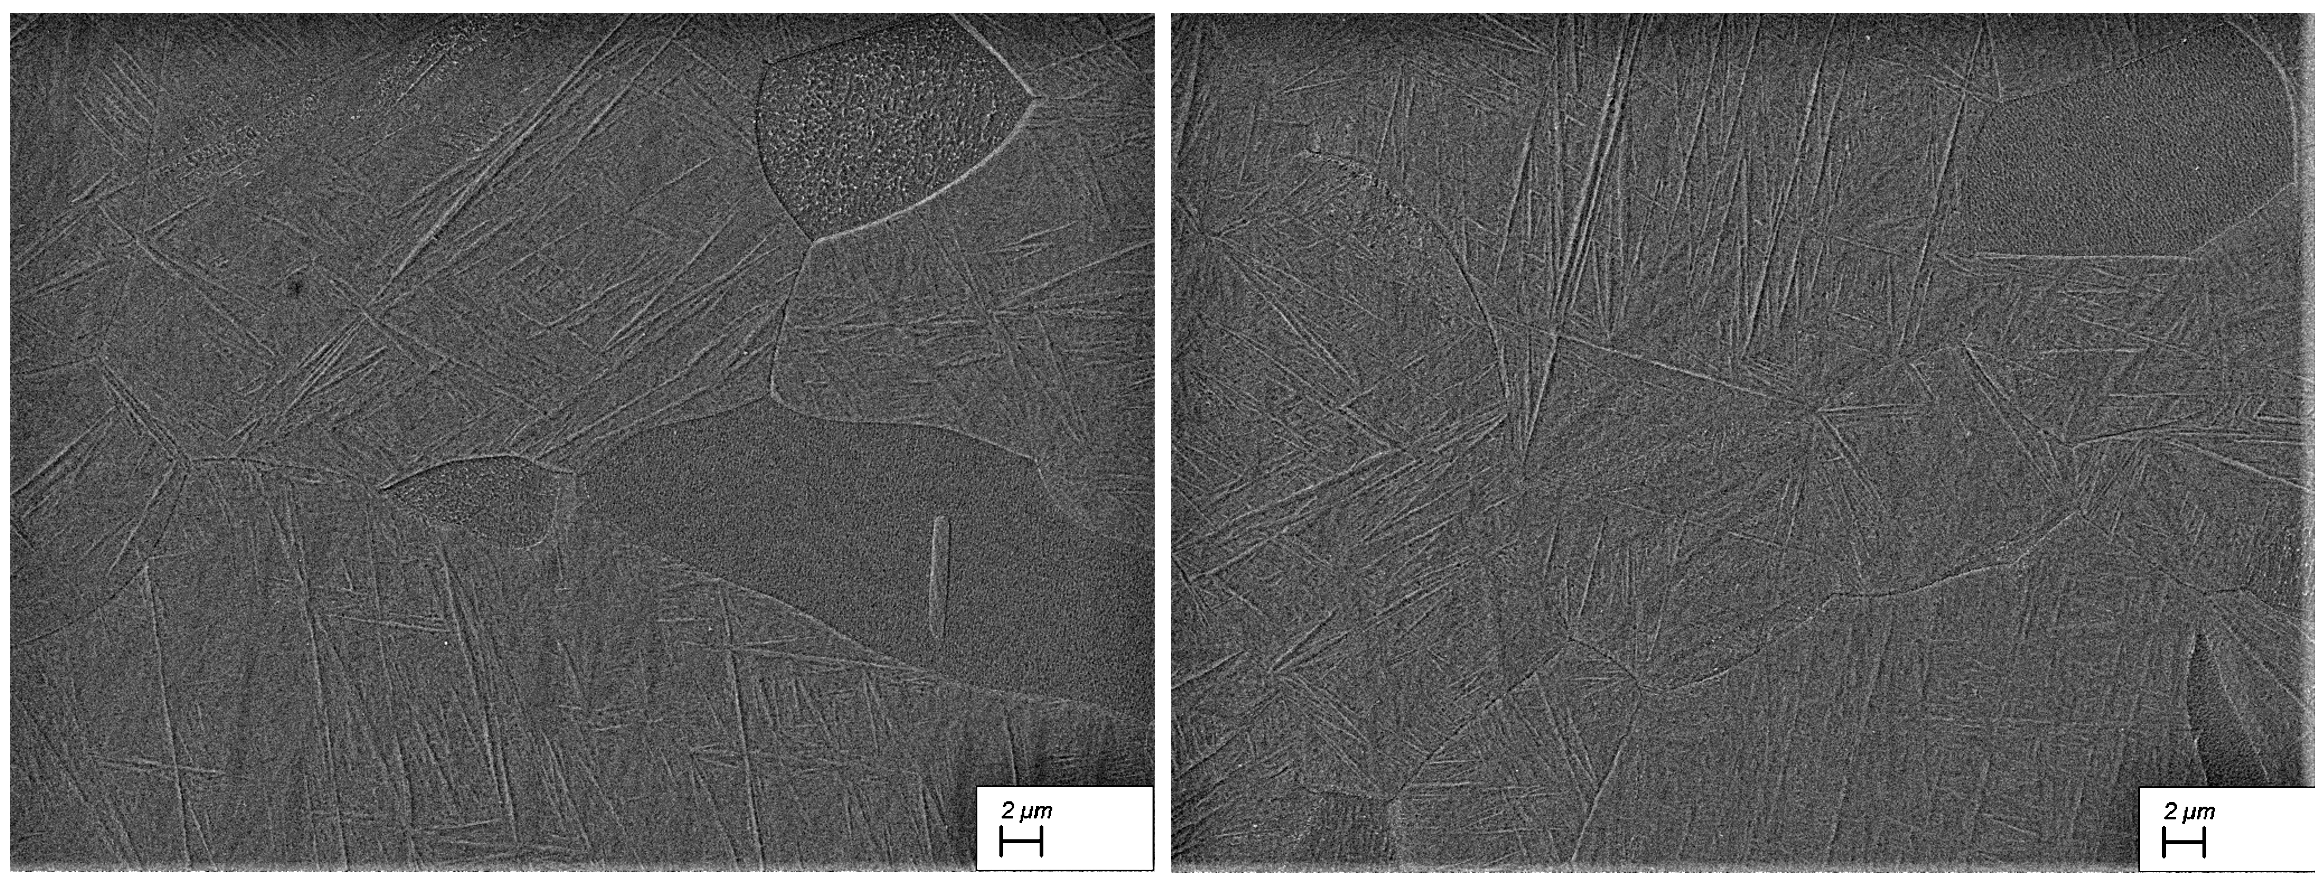
\includegraphics[width=0.9\linewidth]{./Bilder/Abbildung 26.png}
	\caption[Abbildung 26]{983$^\circ$C/1h/WQ + 610$^\circ$C/16min/AC, REM}
	\label{fig:abbildung-26}
\end{figure}

\begin{figure}[h]
	\centering
	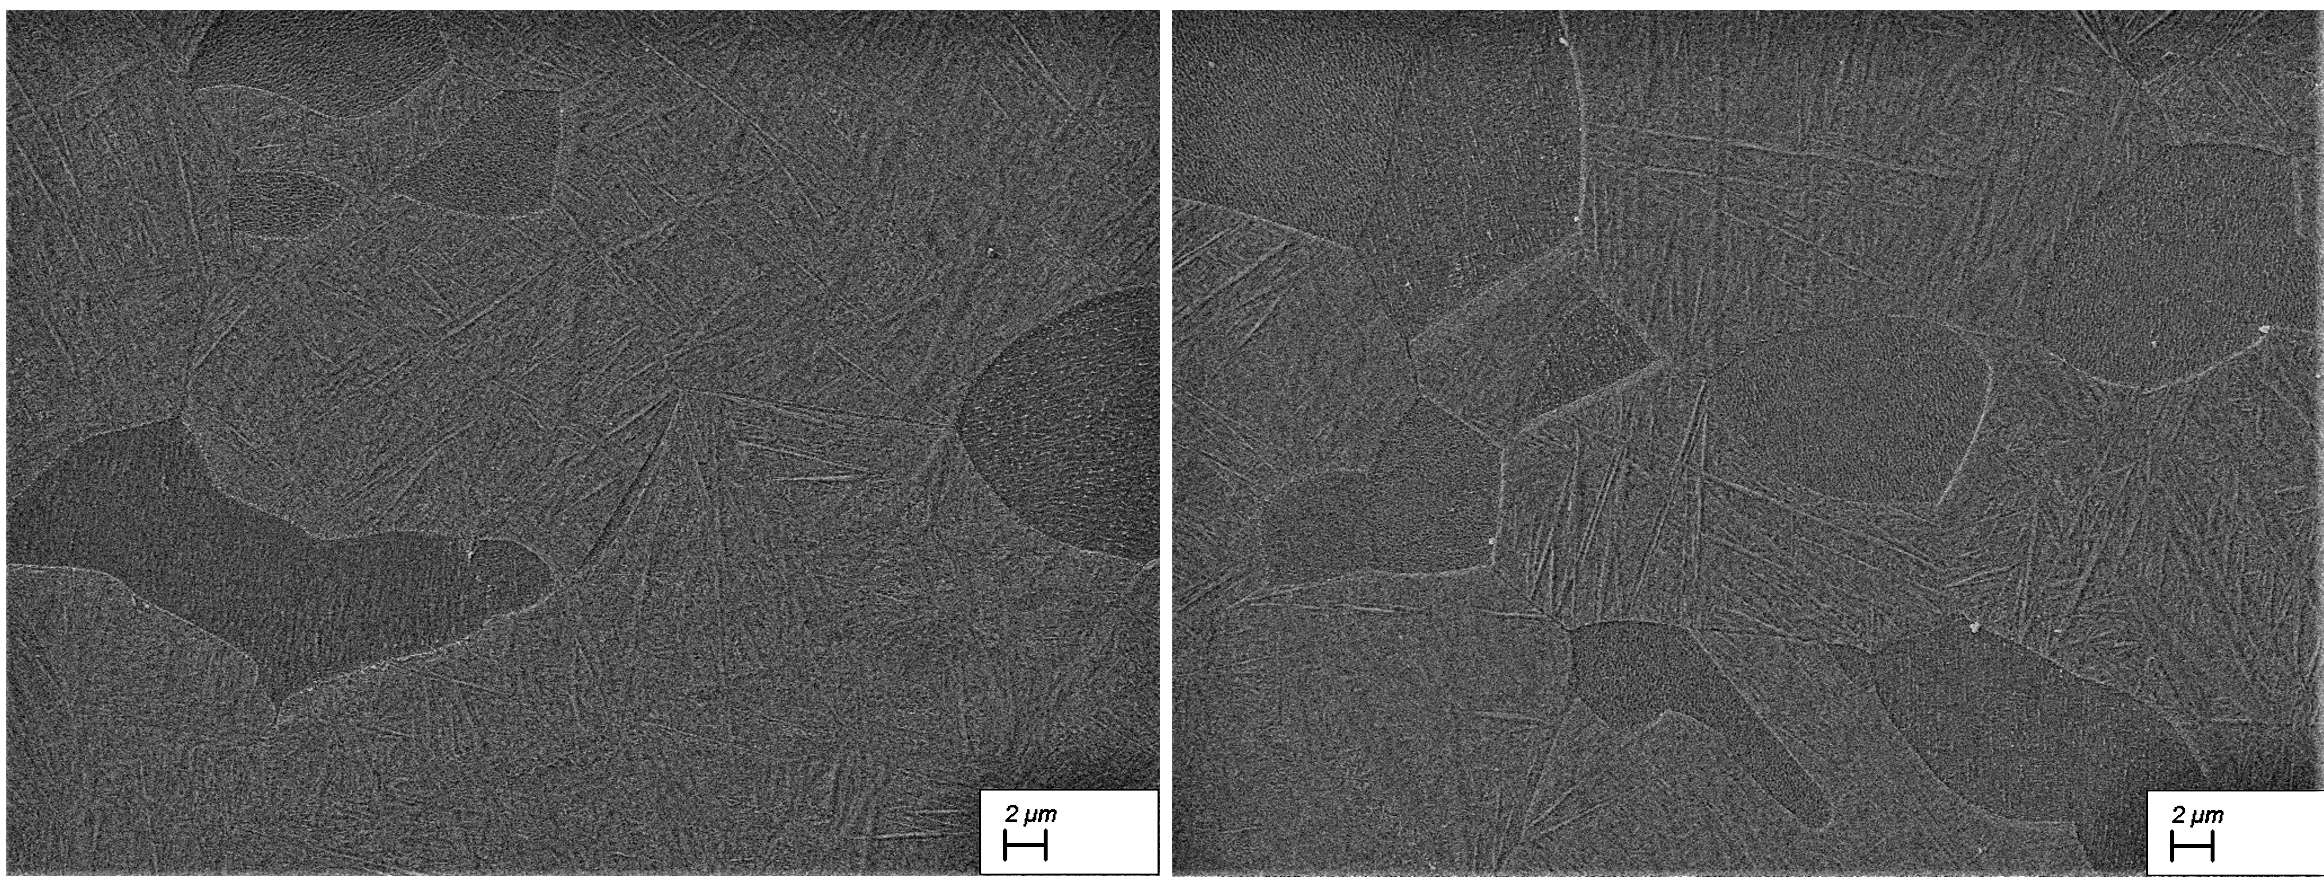
\includegraphics[width=0.9\linewidth]{./Bilder/Abbildung 27.png}
	\caption[Abbildung 27]{983$^\circ$C/1h/WQ + 610$^\circ$C/30min/AC, REM}
	\label{fig:abbildung-27}
\end{figure}

In den Abbildungen \ref{fig:abbildung-26} und \ref{fig:abbildung-27} ist zu erkennen, dass keine Veränderung in dem Gefüge im Vergleich zum vorherigen Schritt feststellbar ist. Es kann davon ausgegangen werden, dass der geplante Martensitzerfall nicht stattgefunden hat.

Die Ergebnisse der Härteprüfung nach diesem zweiten Schritt sind in Tabelle \ref{Tabelle 9} aufgeführt.

\begin{table}[h]
	\centering
	\begin{tabular}{|c|c|}
		\hline 
		Probe & Härte in HV \\ 
		\hline 
		983$^\circ$C/1h/WQ + 610$^\circ$C/16min/AC & 405 \\ 
		\hline 
		983$^\circ$C/1h/WQ + 610$^\circ$C/30min/AC & 400 \\ 
		\hline 
	\end{tabular} 
	\caption{Ergebnisse der Härteprüfung nach der zweiten Wärmebehandlung, $\alpha_p$- $\alpha'$-Gefüge}
	\label{Tabelle 9}
\end{table}

Es ist zu erkennen, dass auch die Härte unverändert im Vergleich zum vorherigen Schritt blieb.

\section{Diskussion (ZB)}

\paragraph{Glühen und Abschrecken}
Vor dem Abschrecken stellt sich ein zweiphasiges Gefüge ein ($\alpha$- und $\beta$-Phase). Der große $\beta$-Anteil des Gefüges konnte aber durch die Diffusion von 2\% Molybdän nicht stabilisiert werden und wandelte sich beim Abschrecken martensitisch um. Die Bildung von den Martensit-Nadeln verfeinert das Gefüge. Diese neu geformten Grenzflächen behindern die Versetzungsbewegungen, sodass die Härte dieser Proben von 331 auf 405 HV gestiegen ist. 

\paragraph{Anlassen} Nach dem Anlassen hat sich gezeigt, dass $\alpha'$ nicht zerfallen konnte. Das ist wahrscheinlich darauf zurückzuführen, dass die Haltezeit von 30 min nicht ausreichend für die Umwandlung der Martensitnadeln in  $\beta$ + $\alpha$ war. Eine weitere Erklärung dafür könnte sein, dass diese Transformation bei 610$^\circ$C so langsam ablief, dass sie innerhalb von 30 min nicht stattfinden konnte.
Deshalb waren keine Gefüge- oder Härteänderungen im Vergleich zu dem ersten Schritt festzustellen. 

